% Source of the figure padding.pdf: the graph G with a new vertex u' joined to u by two internally disjoint paths of
% length two through the new vertices s_1 and s_2; the four new edges are the edges of F(u',v). Compile with
% pdfLaTeX; the PDF is included in the manuscript at its natural size.
\documentclass[tikz,border=1pt]{standalone}
\usepackage[T1]{fontenc}
\pdfinfoomitdate=1 \pdftrailerid{} \pdfsuppressptexinfo=-1
\usetikzlibrary{arrows.meta}
\definecolor{fblue}{RGB}{31,102,178}
\tikzset{
  vertex/.style={circle, fill=black, inner sep=0pt, minimum size=2.2mm},
  terminal/.style={circle, fill=black, inner sep=0pt, minimum size=3mm},
  region/.style={rounded corners=10pt, fill=gray!14, draw=gray!75!black, line width=0.9pt},
  fedge/.style={line width=0.9pt, fblue, dash pattern=on 3pt off 1.6pt, -{Stealth[length=2.4mm, width=2mm]}}}
\begin{document}
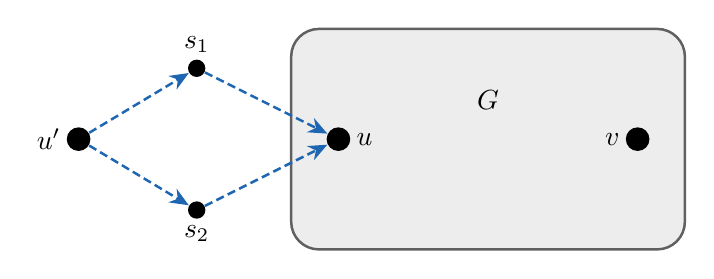
\begin{tikzpicture}[x=1cm, y=1cm]
  % the graph G
  \draw[region] (2.7,-1.4) rectangle (7.7,1.4);
  \node at (5.2,0.5) {$G$};
  \node[terminal] (u) at (3.3,0) {};
  \node[terminal] (v) at (7.1,0) {};
  \node[right=3pt] at (u) {$u$};
  \node[left=3pt]  at (v) {$v$};
  % the new vertices and the four new edges
  \node[terminal] (u1) at (0,0) {};
  \node[vertex]   (s1) at (1.5,0.9)  {};
  \node[vertex]   (s2) at (1.5,-0.9) {};
  \node[left=3pt]  at (u1) {$u'$};
  \node[above=2pt] at (s1) {$s_1$};
  \node[below=2pt] at (s2) {$s_2$};
  \draw[fedge] (u1) -- (s1);
  \draw[fedge] (s1) -- (u);
  \draw[fedge] (u1) -- (s2);
  \draw[fedge] (s2) -- (u);
\end{tikzpicture}
\end{document}
